%\documentclass[noarxiv]{../../latex_styles/quantum/quantumarticle}
%----- Q-SE 2027 submission class ------%
\documentclass[10pt,conference]{IEEEtran}

\usepackage{graphicx}
\usepackage{booktabs}
\usepackage{import}
\usepackage{longtable}
\usepackage{hyperref}
\makeatletter
\@ifclassloaded{quantumarticle}{}{
    \usepackage{tabularx}
    \usepackage{xltabular}
}
\makeatother
\usepackage{listings}
\usepackage{braket}
\usepackage{amssymb}
\usepackage{mdframed}
\usepackage{threeparttable}
\usepackage{amsmath}
\usepackage[T1]{fontenc}
\usepackage{enumitem}
\usepackage{multirow}
\makeatletter
\@ifundefined{frontmatter}{%
  \newcommand{\frontmatter}{\cleardoublepage\pagenumbering{roman}}
}{}
\@ifundefined{mainmatter}{%
  \newcommand{\mainmatter}{\cleardoublepage\pagenumbering{arabic}}
}{}
\@ifundefined{backmatter}{%
  \newcommand{\backmatter}{\cleardoublepage}
}{}

% Define \chapter if not defined (as in article class)
\@ifundefined{chapter}{%
  \newcommand{\chapter}{\section}
}{}

% Retain the complete content unless submission exclusions are enabled.
\@ifundefined{ifthesis}{%
  \newif\ifthesis
  \thesistrue
}{}

% Retain the complete content unless anonymization exclusions are enabled.
\@ifundefined{ifanon}{%
  \newif\ifanon
  \anonfalse
}{}
\makeatother

\usepackage{biblatex}

\addbibresource{bib/references.bib}
\ifanon
    \addbibresource{bib/anon_self_references.bib}
\else
    \addbibresource{bib/self_references.bib}
\fi

% Apply exclusions for non thesis build
\thesisfalse

\begin{document}

    \title{From Assembly to Quantum-Implicit: Characterising the Abstraction Gap in Quantum Programming Systems}
%    \author{
%        \IEEEauthorblockN{
%            Constantinos Kavadias,
%            Udaya Parampalli and
%            Cezary Kaliszyk
%        }
%        \IEEEauthorblockA{
%            University of Melbourne\\
%            ckavadias@student.unimelb.edu.au,
%            udaya@unimelb.edu.au,
%            cezary.kaliszyk@unimelb.edu.au
%        }
%    }
%    \author{Constantinos Kavadias}
%    \email{ckavadias@student.unimelb.edu.au}
%
%    \author{Udaya Parampalli}
%    \email{udaya@unimelb.edu.au}
%
%    \author{Cezary Kaliszyk}
%    \email{cezary.kaliszyk@unimelb.edu.au}

    \maketitle

    \begin{abstract}
        Quantum programming systems simplify implementation but continue to require quantum-specific knowledge.
        Prior classifications surveyed paradigms such as functional and imperative programming without establishing whether representative programs can be written without quantum-mechanical prerequisites.
        This review defines a five-tier abstraction taxonomy spanning Assembly, IR, Framework, High-level and Quantum-implicit, and assesses eleven systems through four representative tasks and nine conditions.
        Primary-source code evidence supports condition outcomes and tier assignments by justified profile match, with explicit quantum-implicit gating constraints.
        No assessed system meets the quantum-implicit requirements across the task suite.
        Although the representative constructions avoid hardware-specific authoring, quantum artefacts, resource identities, observation boundaries and required quantum concepts remain recurring programming obligations.
        Task-local simplifications do not satisfy the complete quantum-implicit profile.
        The findings identify a structural gap across the reviewed approaches, justifying a new quantum programming language that makes quantum realisation a compilation responsibility while preserving optional expert control.
    \end{abstract}

    \section{Introduction}\label{sec:introduction}
Quantum software development has produced languages, frameworks and execution models seeking to reduce programmer friction and improve expressivity~\cite{DiMatteo2024AbstractionHierarchy}.
Productive quantum programming requires separation between a \textit{programming} layer that expresses algorithmic intent, an \textit{execution} layer that determines and optimises its realisation and a \textit{hardware} layer that implements device-specific instructions~\cite{DiMatteo2024AbstractionHierarchy}.
\textit{Bleed-through} occurs when execution- or hardware-layer concerns become obligations at the programming layer~\cite{DiMatteo2024AbstractionHierarchy}.
Circuit-centred authoring requires programmers to specify quantum operations and resources rather than leaving their realisation entirely to the implementation.
Better abstract machines and stronger layer boundaries are therefore proposed as requirements for productive quantum programming~\cite{nunez_corrales2025betterabstractmachines}.

This review examines whether contemporary systems simplify quantum programming or make quantum-specific knowledge non-mandatory.

\subsection{Abstraction and productivity}\label{subsec:introduction:abstraction_productivity}
A comparison of scripting languages (Perl, Python, Rexx and Tcl) with imperative languages (C, C++ and Java) found that scripting-language users completed comparable tasks in roughly half the time and produced solutions half the length~\cite{Prechelt2000EmpiricalComparison}.
These findings motivate examining abstraction, rather than establishing its effect on quantum programming productivity.
Higher-level abstraction has been argued to be necessary for productive quantum programming~\cite{cobb2022higherlevelabstractions}.
The present review examines programming requirements rather than measuring productivity gains.

\subsection{Quantum bias and developer friction}\label{subsec:introduction:quantum_bias}
Programming languages are user interfaces whose design determines the concepts programmers must understand~\cite{Myers2016PLUsabilitySIG}.
This review terms the quantum-specific component of that requirement \textit{quantum bias}: the degree to which gates, qubits, measurement and other quantum-mechanical concerns are required to understand and productively use a language.
Quantum bias remains when ordinary mathematical or computational intent must be reformulated through quantum-specific constructs.

A survey of quantum programmers identified quantum-specific vocabulary and concepts as a challenge, with 31\% of respondents expressing a desire for newer, higher-level languages~\cite{ferreira2024qplusage}.
Analysis of Stack Overflow discussions also reports difficulties integrating classical and quantum components~\cite{stackoverflowqc2026}.
These findings motivate examining quantum-dependent types and constructs, composition across interfaces and explicit resource-management requirements.
The evaluation instrument examines these concerns through representative tasks and conditions concerning artefacts, resource identity, composition, observation and required quantum knowledge.

\subsection{Research questions}\label{subsec:introduction:research_questions}
\begin{description}
    \item[RQ1] What is the current state of abstraction in quantum programming systems, and to what extent do existing systems meet the abstraction requirements identified in prior work on productive quantum programming?
    \item[RQ2] Given the abstraction gap identified in RQ1, is the development of a new quantum programming language targeting higher abstraction justified, or can existing systems be adapted to close the gap?
\end{description}

RQ1 is answered through systematic assessment of eleven systems using four representative tasks and nine evidence-backed conditions.
RQ2 draws on the comparative findings and practitioner evidence to assess the implications for language design~\cite{ferreira2024qplusage}.

\subsection{Contributions}\label{subsec:introduction:contributions}
\begin{enumerate}
    \item A five-tier abstraction taxonomy with explicit quantum-implicit criteria.
    \item An evidence-first evaluation instrument comprising four tasks, nine conditions, expected tier profiles and quantum-implicit gating constraints.
    \item An operationalisation of quantum bias through required concepts and programming obligations.
    \item Systematic assessments of eleven systems, producing condition profiles and comparative findings on abstraction requirements.
    \item Evidence-grounded design implications for quantum-implicit programming.
\end{enumerate}
\section{Background and related work}\label{sec:background}
An early survey classified quantum programming languages by imperative, functional and formal semantic approaches, identifying complex data structures and expressive quantum control as structural gaps~\cite{Gay2006QPLSurvey}.
Its scope preceded contemporary frameworks and excluded hosted quantum libraries on grounds of insufficient language-level formalisation~\cite{Gay2006QPLSurvey}.

A survey of quantum SDKs and frameworks found no consistent progression toward greater separation from the quantum substrate~\cite{furntratt2024higherabstractionlevels}.
An evaluation using lines of code, cyclomatic complexity and Halstead complexity found that higher-level claims did not consistently correspond to lower complexity, nor did standalone languages systematically outperform hosted libraries~\cite{corralesgarro2025productivityexpressiveness}.

A quantum IR review assessed hardware agnosticism, optimisation, tooling accessibility and ease of use~\cite{irreview2024}.
QIR, Q-MLIR and related systems could perform well technically while remaining difficult to access through tooling~\cite{irreview2024}.

These comparisons examine paradigms, code complexity and technical capabilities rather than the cross-tier, task-based account of mandatory quantum vocabulary and programming obligations developed here.

\subsection{Abstraction requirements and documented gaps}\label{subsec:background:abstraction}
Work on quantum abstract machines identifies programming-layer requirements for separating computational intent from quantum implementation.
These include symbolic denotational syntax, representation-independent data types and a stable instruction set architecture, which no examined candidate jointly satisfies~\cite{nunez_corrales2025betterabstractmachines}.
The analysis identifies coupling between instruction symbols and circuit primitives and proposes an application-programming target independent of qubit modality and gate-set choice~\cite{nunez_corrales2025betterabstractmachines}.

Quantum semantics constrain how implementations achieve that separation.
No-cloning restricts copying, observation can change quantum data and temporary computations require a reversible clean-up account~\cite{yuan2025foundationalabstractions}.
Classical control constructs cannot transfer unrestrictedly to superposition while preserving unitary behaviour~\cite{yuan2025foundationalabstractions}.
These constraints must be respected by implementations but do not by themselves determine which obligations remain visible to programmers.

Among 251 surveyed quantum programmers, 86\% had at least five years of classical programming experience, yet quantum-specific vocabulary remained a prominent challenge~\cite{ferreira2024qplusage}.
Substantial classical programming experience therefore does not remove the need to learn quantum-specific concepts.
The review examines those requirements directly rather than treating improved tooling, language packaging or reduced code complexity as sufficient evidence of abstraction.

\subsection{Programming language usability frameworks}\label{subsec:background:usability}
PLIERS grounds programming language evaluation in language goals and intended users' requirements~\cite{Coblenz2021PLIERS}.
This review applies that goal-oriented approach to characterise required programmer knowledge through representative tasks.
The assessment concerns interface obligations rather than measured onboarding, productivity or error rates, which require subsequent human-factors validation.

\ifthesis
\subsection{Systematic review methodology}\label{subsec:background:slr}
Software engineering systematic reviews use pre-specified questions and procedures, explicit eligibility criteria, documented searches, quality assessment and structured synthesis to support reproducibility and audit~\cite{KitchenhamCharters2007SLR}.
Narrative synthesis accommodates heterogeneous evidence where meta-analysis is inappropriate~\cite{KitchenhamCharters2007SLR}.
PRISMA 2020 supplies reporting conventions for transparent accounts of identification, selection, methods and findings~\cite{page2021prisma}.

The earlier comparisons discussed here remain useful within their stated scopes.
Their descriptions of systems, complexity measures and tier-specific criteria do not provide the complete protocol and evidence trail required for the present cross-tier assessment.
Section~\ref{sec:methodology} specifies this review's search, screening, extraction, quality and synthesis procedures, with the protocol and supporting records supplied as linked artefacts.

The contribution is a common evidential basis for locating the reviewed systems relative to explicit quantum-implicit requirements.
It combines literature-derived abstraction criteria with representative tasks and traceable condition outcomes.
The resulting comparison distinguishes obligations that systems simplify, obligations they remove in particular tasks and obligations that remain across the assessed suite.
\fi
\section{Taxonomy of quantum programming systems}\label{sec:taxonomy}
The taxonomy distinguishes programmer-facing abstraction through programming requirements, primary artefacts and allocation of implementation responsibility, following the programming, execution and hardware separation identified in prior work~\cite{DiMatteo2024AbstractionHierarchy}.

Tier definitions concern what programmers must understand and author, not merely what a system can produce.
Descriptive system roles do not determine assessed tiers, which depend on representative programming evidence.

\begin{description}
    \item[Assembly (A)]
    Explicit gates, measurements and classical control operate on visible qubit registers for interchange and execution~\cite{cross2022openqasm3}.
    Hardware control is exposed; portability follows instruction semantics rather than data abstraction.

    \item[Intermediate representation (IR)]
    Compiler and tooling representations support interchange, lowering, optimisation and analysis, exposing qubit lifetime and quantum/classical distinctions~\cite{qir_alliance_qir_spec_repo,McCaskey2021MLIRDialectQASM}.
    Compilation role, not a fixed stack position, defines the tier.

    \item[Framework (FW)]
    Reusable quantum operations are organised through library APIs or language constructs, while representative programming retains circuit manipulation, explicit register management or staging obligations.

    \item[High-level (HL)]
    Quantum-explicit functions, modules and types replace circuit-file authoring.
    Safety disciplines govern resources and clean-up, with compiler assistance and optional hardware tuning.

    \item[Quantum-implicit (QI)]
    This tier operationalises literature-derived requirements for programming abstractions independent of quantum realisation~\cite{nunez_corrales2025betterabstractmachines}.
    Ordinary mathematical and computational abstractions require no quantum-mechanical vocabulary.
    The implementation infers quantum realisation, lowers it to IR or circuits and manages results without a programmer-visible observation boundary.
    Expert control, optimisation and hardware tuning remain opt-in.
\end{description}

\ifthesis
\begin{mdframed}[frametitle={Litmus test}]
    A language is quantum-implicit if a programmer with no prior instruction in quantum mechanics can learn it from its own documentation.
    That programmer must be able to implement representative programs without needing to understand qubits, gates, amplitudes or entanglement.
\end{mdframed}
\fi

Section~\ref{sec:evaluation_instrument} operationalises these requirements through representative tasks, condition profiles and explicit gating constraints.

\ifthesis

\subsection{Systems under review}\label{subsec:taxonomy:systems}
Table~\ref{tab:taxonomy:systems} identifies eleven primary systems selected under the criteria in Section~\ref{sec:methodology}, with per-system verification in Appendix~B of~\cite{kavadias2026qplSurveySupplementary}.
Tower is included as an unassessed comparison.
Artefact types are descriptive; assessed tiers are reported in Section~\ref{sec:system_assessments}.

\begin{table}[htbp]
    \centering
    \caption{Systems under review. Artefact types are descriptive; assessed tier assignments are reported in Section~\ref{sec:system_assessments}.}
    \label{tab:taxonomy:systems}
    \begin{threeparttable}
        \footnotesize
        \begin{tabular}{ll}
            \toprule
            \textbf{System}                                           & \textbf{Artefact type}       \\
            \midrule
            OpenQASM~3.0~\cite{cross2022openqasm3}                    & Circuit description language \\
            \addlinespace
            QIR~\cite{qir_alliance_qir_spec_repo}                     & Compiler IR                  \\
            \addlinespace
            Q-MLIR~\cite{McCaskey2021MLIRDialectQASM}                 & Compiler IR                  \\
            \addlinespace
            Qiskit~\cite{aleksandrowicz2019qiskit}                    & Embedded circuit framework   \\
            \addlinespace
            PennyLane~\cite{bergholm2018pennylane}                    & Embedded circuit framework   \\
            \addlinespace
            Q\#~\cite{MicrosoftQSharpOverview}                        & Standalone QPL               \\
            \addlinespace
            Silq~\cite{bichsel2020silq}                               & Standalone QPL               \\
            \addlinespace
            Qmod~\cite{vax2025qmodexpressivehighlevelquantum}         & Standalone QPL               \\
            \addlinespace
            Quff~\cite{wright2024quff}                                & Standalone QPL               \\
            \addlinespace
            Qutes~\cite{faro2025qutes,reversiblelifetime2026}         & Standalone QPL               \\
            \addlinespace
            Qwerty~\cite{adams2024qwerty}                             & Standalone QPL               \\
            \addlinespace
            Tower~\cite{yuan2025foundationalabstractions}\tnote{\dag} & Standalone QPL               \\
            \bottomrule
        \end{tabular}
        \begin{tablenotes}
            \footnotesize
            \item[\dag] Unassessed and provided for comparison only\ifthesis; see Section~\ref{subsec:system_descriptions:tower}.\else.\fi
        \end{tablenotes}
    \end{threeparttable}
\end{table}
\fi
\section{Evaluation instrument}\label{sec:evaluation_instrument}
The evaluation instrument operationalises the taxonomy in Section~\ref{sec:taxonomy} through four representative programming tasks and nine conditions.
Tier assignment follows a justified match between evidence-backed condition profiles and expected tier profiles, subject to explicit quantum-implicit gating constraints.

\ifthesis

\subsection{Evaluation lenses}\label{subsec:evaluation_instrument:lenses}
Five lenses guide interpretation of the programming evidence.
\begin{description}
    \item[Required mental model and vocabulary] The quantum-mechanical and execution-model concepts required to complete representative workflows.
    \item[Primary artefact] The object the programmer authors or manipulates: a program over values or an explicit circuit, tape, IR or graph.
    \item[Safety discipline and semantic guarantees] The enforced type or effect discipline, including linearity, affinity, uncomputation and validity constraints~\cite{pierce2002tapl-doc9,bichsel2020silq}.
    \item[Compilation responsibility] The division of obligations between the programmer and compiler or runtime, including quantum structure, resource management and clean-up.
    \item[Execution and hardware adjacency] The visibility of basis gates, timing, controller instructions and device-specific constraints.
\end{description}

\textit{Bleed-through} occurs when execution- or hardware-layer concerns surface at the programming layer, requiring quantum-native vocabulary even where the programmer's intent could be expressed without it~\cite{DiMatteo2024AbstractionHierarchy,nunez_corrales2025betterabstractmachines}.
Required lower-layer obligations inform negative or constrained condition outcomes.

The mental-model lens informs conditions concerning superposition, marking and required quantum concepts.
The primary-artefact lens informs circuit-centric authoring and composition.
Safety and compilation responsibility inform uncomputation, while hardware adjacency informs execution constraints.
The lenses guide interpretation rather than being assessed directly; tier assignment depends on the evidenced condition profile.
\fi

\subsection{Representative task suite}\label{subsec:evaluation_instrument:task_suite}
Representative tasks ground evaluation in concrete programmer intent~\cite{Myers2016PLUsabilitySIG}.
Following PLIERS, four tasks were defined before evaluation to reflect real workflows and use each language's primary surface model rather than optional escape hatches~\cite{Coblenz2021PLIERS}.

\begin{description}
    \item[$T_1$ Deutsch--Jozsa]
    Parameterise the decision procedure for small $n$, supply an explicit oracle or intended oracle hook with a balanced oracle by default and execute it to expose a decision artefact.

    \item[$T_2$ Grover search]
    Define a simple marked-state or predicate oracle and implement one or a small fixed number of complete iterations, each comprising oracle phase flip and diffusion.
    Provide the canonical execution and result-extraction pathway.

    \item[$T_3$ Quantum phase estimation]
    For a small unitary $U$ with known phase or eigenvalue and small precision $t$, implement controlled-$U^{2^k}$ for $k=0,\ldots,t-1$ and an explicit inverse QFT or cited library routine.
    Expose estimated phase bits or a documented analogue.

    \item[$T_4$ Bell state preparation]
    Define or call a reusable routine preparing an entangled pair from $\ket{00}$ and demonstrate follow-on use by another routine or an additional controlled operation.
    Avoid measurement in the core construction where possible.
\end{description}

For every task, required measurement, sampling, shots or observable-boundary concepts are recorded in the condition outcomes, including where the system requires observation to expose the Bell construction's result.
Tasks provide evidence for condition outcomes rather than scoring items.

\subsection{Conditions and outcome labels}\label{subsec:evaluation_instrument:conditions}
Each system and task is assessed against the nine conditions in Table~\ref{tab:evaluation_instrument:expected_profile}.
\textbf{Fail (F)} indicates the condition is not met.
\textbf{Constrained (C)} indicates the condition is met only partially or under restrictions, with some quantum-specific programming obligations remaining explicit.
\textbf{Pass (P)} indicates the condition is met in the representative programming model.

Table~\ref{tab:evaluation_instrument:expected_profile} defines the nine conditions and gives their expected outcomes by tier.

\begin{table*}[t]
    \centering
    \caption{Conditions and expected outcomes in representative $T_1$--$T_4$ constructions.
    Bold entries identify mandatory QI gating outcomes.}
    \label{tab:evaluation_instrument:expected_profile}
    \footnotesize
    \setlength{\tabcolsep}{3pt}
    \begin{tabular}{lp{0.70\textwidth}ccccc}
        \toprule
        \textbf{ID} & \textbf{Definition}                                                                                                                                             & \textbf{A} & \textbf{IR} & \textbf{FW} & \textbf{HL} & \textbf{QI}  \\
        \midrule
        $C1$        & \textbf{Superposition as a value.} Introduced without explicit qubit identity or gate-level initiation as the conceptual entry point. & $F$ & $F$ & $F$ & $C$ & $P$ \\
        $C2$        & \textbf{Primary artefact.} Programs over values, not construction or manipulation of circuits, tapes, IRs or graph objects. & $F$ & $F$ & $F$ & $C$ & $\mathbf{P}$ \\
        $C3$        & \textbf{Resource identity and lifetime.} No required qubit handles, allocation, indexing, lifetime management, reset or release. & $F$ & $F$ & $F$ & $C$ & $\mathbf{P}$ \\
        $C4$        & \textbf{Uncomputation not manual reverse-programming.} Clean-up is automatic or structured rather than requiring manual inversion as a normal correctness step. & $F$ & $F$ & $F$ & $C$ & $P$ \\
        $C5$        & \textbf{Quantum/classical boundaries.} No mandatory explicit marking or staging between quantum and classical computation. & $F$ & $F$ & $C/F$ & $C$ & $P$ \\
        $C6$        & \textbf{Observation boundary.} Results require no explicit measurement, sampling, shots or observable-boundary concepts. & $F$ & $F$ & $F$ & $C$ & $\mathbf{P}$ \\
        $C7$        & \textbf{Hardware separation.} No required basis gates, topology, timing or backend constraints; tuning remains opt-in. & $F$ & $C$ & $P$ & $P$ & $P$ \\
        $C8$        & \textbf{Required quantum knowledge.} Correctness requires no direct reasoning about amplitudes, phases, entanglement or interference. & $F$ & $F$ & $C/F$ & $C$ & $P$ \\
        $C9$        & \textbf{Subroutine composition.} Larger programs compose subroutines rather than requiring circuit surgery or staging glue. & $F$ & $F$ & $C$ & $P$ & $\mathbf{P}$ \\
        \bottomrule
    \end{tabular}
\end{table*}

C4 outcomes are read primarily from T1--T3, whose oracle, diffusion and controlled-power constructions exercise auxiliary-state clean-up.
Bell preparation does not require uncomputation in its core construction.
C6 is read from the worst case across T1--T4: Bell preparation can avoid measurement internally, while the algorithmic tasks generally require result extraction.

C2, C3 and C6 are the principal discriminators between High-level and Quantum-implicit.
Quantum-implicit classification requires $C2$, $C3$, $C6$ and $C9$ to pass in representative $T_1$--$T_4$ constructions.
These conditions are necessary but not sufficient.
\section{Review methodology}\label{sec:methodology}
The review follows evidence-based software engineering guidelines~\cite{KitchenhamCharters2007SLR}, with a pre-registered protocol available at~\cite{kavadias2026qplSurveyProtocol}.

\subsection{Search protocol}\label{subsec:methodology:search_protocol}
Searches were conducted on 2026-05-19 across ACM Digital Library, IEEE Xplore and arXiv, with a literature cutoff of 2026-04-08.
Official project and specification sites were consulted per system throughout assessment; later evidence was excluded.

Three verbatim search strings were applied consistently across the databases:
\begin{description}
    \item[S1: broad seed terms] \texttt{"quantum programming language" OR "quantum intermediate representation" OR OpenQASM OR "quantum MLIR" OR Silq OR Qiskit OR PennyLane}.
    \item[S2: system-specific terms] \texttt{Silq quantum OR Quff quantum OR Qutes quantum OR Quipper quantum OR "Microsoft Q\#" OR "Q-MLIR"}.
    \item[S3: abstraction framing] \texttt{"quantum programming" AND "abstraction" AND "language"}.
\end{description}
The searches retrieved 852 records from arXiv, 1{,}295 from ACM Digital Library and 704 from IEEE Xplore.
The combined 2{,}851 records yielded 2{,}233 unique records after deduplication.
Per-database counts, search strings and URLs are published in Appendix~A of~\cite{kavadias2026qplSurveySupplementary}.

Supplementary AI-assisted discovery used a scheduled agent to surface candidates from project context fortnightly.
Its dynamically generated queries are not reproducible verbatim and do not constitute a primary database search.
All candidates underwent the same eligibility screening.

\subsection{Screening and selection}\label{subsec:methodology:screening}
A bounded, pre-specified seed set informed search design and validation.
Database searches provided primary discovery; extraction concerns included systems' authoritative papers, specifications and documentation rather than the full retrieved corpus.

Systems must satisfy at least three of four inclusion criteria:
\begin{description}
    \item[$C_1$] A formal specification or peer-reviewed primary paper exists.
    \item[$C_2$] Active releases or specification updates within 24 months prior to the cutoff.
    \item[$C_3$] Multivendor or multi-device backend support beyond a single lab or vendor.
    \item[$C_4$] Public documentation is enough to complete the representative tasks defined in Section~\ref{subsec:evaluation_instrument:task_suite} without access to private knowledge.
\end{description}
Exclusions comprise marketing-only primary materials, projects inactive for more than 36 months and documentation insufficient for representative workflows.
Assessment uses the latest stable major release or specification available at the cutoff; earlier versions serve only as labelled historical contrasts.

Screening was conducted by one reviewer, with full-text exclusion rationales in Appendix~B of~\cite{kavadias2026qplSurveySupplementary}.
Two additional reviewers participated in independent assessment and calibration reconciliation.
The bounded review did not permit dual screening of the full inclusion corpus, which remains a review-process limitation~\cite{page2021prisma}.

\subsection{Evidence quality, extraction and synthesis}\label{subsec:methodology:quality}
Source quality was assessed before extraction using a hierarchy adapted from evidence-based software engineering guidelines~\cite{KitchenhamCharters2007SLR}.
Tier~1 comprises peer-reviewed journal or conference publications, tier~2 preprints from established groups with a peer-reviewed publication programme and tier~3 official specifications, standards-body publications and maintained documentation.
No included system depends primarily on tier~4 grey literature.
The non-tier~1 primary sources are QIR's official specification, classified as tier~3~\cite{qir_alliance_qir_spec_repo}, and Qmod's preprint, classified as tier~2~\cite{vax2025qmodexpressivehighlevelquantum}.

Each system and task $T_1$--$T_4$ is assessed against $C_1$--$C_9$ using the outcome labels in Section~\ref{sec:evaluation_instrument}.
Outcomes are supported by minimal code constructions, primary-source citations and one-sentence justifications.

Canonical examples from primary papers, specifications, official documentation and tutorials take precedence.
Constructed examples are used only where no canonical example exists for the task or feature.
They are labelled and require primary-source justification for every non-trivial feature.
Abridgement may omit cited routines or helpers outside the evidence claim, but must not conceal the assessed mechanism.

Records capture example type, sources, code, version preconditions, outcomes, justifications and required low-level interfaces.
Outcomes inferred from examples marked optional or advanced were not used.
Absent or ambiguous evidence received the more conservative outcome label.
Appendices~C and~D publish the extraction dataset and assessed code samples respectively~\cite{kavadias2026qplSurveySupplementary}.

Structured narrative synthesis groups systems by taxonomy tier without meta-analysis~\cite{KitchenhamCharters2007SLR}.
Tier assignments are justified by discriminating conditions, condition profiles and cited representative evidence.

\subsection{Sensitivity analysis and threats to validity}\label{subsec:methodology:sensitivity}
Pre-specified leave-one-out analysis examined sole or pivotal source dependencies~\cite{kavadias2026qplSurveyProtocol}.

All Quff outcomes depend on one peer-reviewed paper, with no additional published specification or paper available at the cutoff~\cite{wright2024quff}.
Removing it leaves no evidence base; its outcomes are retained with this dependency acknowledged.

Two tier-relevant Qutes outcomes depend critically on a reversible-lifetime preprint~\cite{reversiblelifetime2026}.
The HPDC~2025 paper alone would not sustain the same tier justification~\cite{faro2025qutes}.
The mechanism's preprint status remains a limitation.

The principal validity threats and mitigations are:
\begin{itemize}
    \item \textit{Assessment subjectivity}: independent assessment, calibration, evidence quotes and predefined rules for ambiguity.
    \item \textit{Task-suite dependence}: protocol-defined tasks and documented, prospective post-calibration amendments~\cite{kavadias2026qplSurveyProtocol}.
    \item \textit{Ecosystem maturity}: source tiers and per-claim confidence ratings.
    \item \textit{Version churn}: consistent assessment of stable releases available by 2026-04-08.
    \item \textit{Publication bias}: specifications and maintainer documentation reduce the risk of under-representing IR-tier and industry-produced frameworks~\cite{KitchenhamCharters2007SLR,page2021prisma}.
    \item \textit{Evidence availability and representativeness}: uneven canonical coverage requires constructed examples, which can over-approximate idiomatic workflows.
    These are labelled, supported by primary sources and document required low-level operations.
    \item \textit{Interpretation drift}: common condition ladders, shared-subset calibration, outcome justifications and conservative treatment of ambiguous evidence.
\end{itemize}
\ifthesis
\section{System descriptions}\label{sec:system_descriptions}
Eleven systems are included under the criteria defined in Section~\ref{sec:methodology}.
The descriptions identify their programming models and mechanisms without assigning assessed tiers.
Tower is retained as a data-abstraction comparison but excluded from primary assessment because it does not satisfy inclusion criteria C\textsubscript{2} and C\textsubscript{4}.

\subsection{OpenQASM 3.0}\label{subsec:system_descriptions:openqasm}
\textbf{OpenQASM 3.0} is a quantum assembly language for circuit interchange and hybrid quantum--classical execution descriptions~\cite{cross2022openqasm3}.
Programmers specify qubit registers, gates, measurements and classical control, including real-time feed-forward~\cite{cross2022openqasm3}.
The optional \texttt{defcal} mechanism supplies pulse-level calibration, while vendor toolchains resolve hardware-specific gate sets and timing constraints~\cite{cross2022openqasm3}.

\subsection{QIR}\label{subsec:system_descriptions:qir}
\textbf{QIR} (Quantum Intermediate Representation) is an LLVM-based compiler and tooling target connecting higher-level quantum languages to backend code generation~\cite{qir_alliance_qir_spec_repo,microsoft_qir_overview}.
Quantum operations use intrinsic calls following QIR conventions, with qubits and measurement results represented as opaque resource types~\cite{qir_alliance_qir_spec_repo}.
The representation supports optimisation, analysis and interoperability across frontends~\cite{qir_alliance_qir_spec_repo,microsoft_qir_overview}.

\subsection{Q-MLIR}\label{subsec:system_descriptions:qmlir}
\textbf{Q-MLIR} denotes MLIR-based quantum intermediate representations that preserve higher-level structure before progressive lowering~\cite{McCaskey2021MLIRDialectQASM}.
Operations cover register allocation and deallocation, qubit addressing, gates and function composition~\cite{McCaskey2021MLIRDialectQASM}.
Static single assignment exposes dataflow, while MLIR passes rewrite quantum dialect operations toward LLVM-compatible and QIR-compliant targets~\cite{McCaskey2021MLIRDialectQASM}.

\subsection{Qiskit}\label{subsec:system_descriptions:qiskit}
\textbf{Qiskit} is an open-source Python quantum-computing SDK developed by IBM Quantum~\cite{aleksandrowicz2019qiskit}.
Its primary authoring artefact is a circuit object constructed through library APIs~\cite{aleksandrowicz2019qiskit}.
Algorithm libraries, transpilation and optimisation passes, simulator and hardware interfaces, and OpenQASM interchange support the path from circuit construction to execution~\cite{aleksandrowicz2019qiskit}.

\subsection{PennyLane}\label{subsec:system_descriptions:pennylane}
\textbf{PennyLane} is a Python framework for differentiable hybrid quantum--classical computation~\cite{bergholm2018pennylane}.
Quantum subroutines are encapsulated as QNodes, which compose with classical code and support automatic differentiation~\cite{bergholm2018pennylane}.
A device-agnostic plugin architecture supports simulators and hardware, with gradients obtained through simulator backpropagation or hardware-compatible parameter-shift rules~\cite{bergholm2018pennylane}.

\subsection{Q\#}\label{subsec:system_descriptions:qsharp}
\textbf{Q\#} is Microsoft's standalone quantum programming language~\cite{MicrosoftQSharpOverview}.
Programmers allocate qubits with \texttt{use}, define typed quantum operations and explicitly reset qubits to $\ket{0}$ before release~\cite{MicrosoftQSharpOverview}.
Functor annotations enable compiler-generated controlled and adjoint variants for structured composition without manually duplicating inverse gate sequences~\cite{MicrosoftQSharpOverview}.

\subsection{Silq}\label{subsec:system_descriptions:silq}
\textbf{Silq} is a statically typed quantum language with safe automatic uncomputation~\cite{bichsel2020silq}.
The compiler frees temporary quantum values where the type discipline establishes that this is safe~\cite{bichsel2020silq}.
Annotations distinguish classically describable functions, read-only inputs and measurement-free functions; quantum values without \texttt{const} follow a linear discipline~\cite{bichsel2020silq}.
The \texttt{reverse} primitive provides circuit inversion~\cite{bichsel2020silq}.

\subsection{Qmod}\label{subsec:system_descriptions:qmod}
\textbf{Qmod} is Classiq's quantum modelling language, available through standalone and Python-embedded interfaces~\cite{vax2025qmodexpressivehighlevelquantum}.
Typed quantum functions operate on explicitly allocated quantum values, including numeric, bit, array and structured types~\cite{vax2025qmodexpressivehighlevelquantum}.
Arithmetic operators act over superpositions, while \texttt{within-apply} structures reversible operations around a target computation and provides automatic uncomputation~\cite{vax2025qmodexpressivehighlevelquantum}.

\subsection{Quff}\label{subsec:system_descriptions:quff}
\textbf{Quff} is a dynamically typed quantum language implemented on GraalVM/Truffle~\cite{wright2024quff}.
Its \texttt{invertF} primitive provides runtime function inversion without programmer-written adjoint circuits~\cite{wright2024quff}.
Dependency-based intermediate representations enable lazy evaluation and deferred quantum type resolution, with quantum typing propagated through expressions containing quantum operands~\cite{wright2024quff}.
Runtime uncomputation is triggered when quantum variables leave scope~\cite{wright2024quff}.

\subsection{Qutes}\label{subsec:system_descriptions:qutes}
\textbf{Qutes} is an imperative quantum language compiled to Qiskit circuits~\cite{faro2025qutes}.
It provides \texttt{qubit}, \texttt{quint} and \texttt{qustring} types, with implicit measurement when quantum variables enter classical contexts~\cite{faro2025qutes}.
The \texttt{in} substring predicate hides Grover-based amplitude amplification~\cite{faro2025qutes}.
Scope-bounded, liveness-guided uncomputation uses dependency and entanglement analysis to insert adjoint operations at safe reclamation points~\cite{faro2025qutes,reversiblelifetime2026}.

\subsection{Qwerty}\label{subsec:system_descriptions:qwerty}
\textbf{Qwerty} is a basis-oriented quantum language that exposes measurement bases and basis changes as programming constructs~\cite{adams2024qwerty}.
Basis information is a first-class concern in the preparation, transformation and observation of quantum values~\cite{adams2024qwerty}.
Its dedicated compiler, \textbf{ASDF}, implements a lowering and optimisation pipeline for basis-oriented programs~\cite{adams2025asdf}.

\subsection{Tower}\label{subsec:system_descriptions:tower}
\textbf{Tower} provides familiar data structures whose operations execute in superposition, paired with a control machine model that removes circuit primitives from the programming surface~\cite{yuan2025foundationalabstractions}.
Reversibility remains explicit through \texttt{assign}/\texttt{unassign} sequencing and \texttt{with-do} constructs, while recursive bounds are supplied as classical parameters~\cite{yuan2025foundationalabstractions}.
\fi
\section{System assessments}\label{sec:system_assessments}
Table~\ref{tab:system_assessments:system_summary} reports tier assignments and aggregated outcomes for eleven systems.
Appendices~C and~D publish extraction data and assessed code~\cite{kavadias2026qplSurveySupplementary}.
Tower is excluded from primary assessment.
Constructed examples comprise OpenQASM T1--T2; QIR T1--T3; Q-MLIR and Quff T1, T3 and T4; Q\# and Qmod T3; and Silq and Qutes T3--T4.

\begin{table}[htbp]
    \centering
    \caption{System assessment result rubric.}
    \label{tab:system_assessments:system_summary}
    \footnotesize
    \setlength{\tabcolsep}{2pt}
    \begin{tabular}{@{}llccccccccc@{}}
        \toprule
        \textbf{Tier} & \textbf{System} & \textbf{C1} & \textbf{C2} & \textbf{C3} & \textbf{C4} & \textbf{C5} & \textbf{C6} & \textbf{C7} & \textbf{C8} & \textbf{C9} \\
        \midrule
        A             & OpenQASM 3.0    & F           & F           & F           & F           & F           & F           & P           & F           & F           \\
        \midrule
        \multirow{IR}
        & QIR             & F           & F           & F           & F           & F           & -           & P           & F           & F           \\
        & Q-MLIR          & F           & F           & F           & F           & F           & F           & P           & F           & C           \\
        \midrule
        \multirow{FW}
        & Qiskit          & F           & F           & F           & F           & F           & F           & P           & F           & C           \\
        & PennyLane       & F           & F           & F           & F           & F           & F           & P           & F           & C           \\
        & Q\#             & F           & F           & F           & C           & F           & F           & P           & F           & C           \\
        & Quff            & F           & C           & F           & C           & C           & C           & P           & F           & P           \\
        & Qutes           & F           & C           & F           & C           & C           & C           & P           & F           & P           \\
        & Qwerty          & C           & C           & C           & C           & F           & F           & P           & F           & P           \\
        \midrule
        \multirow{HL}
        & Silq            & F           & C           & C           & C           & C           & C           & P           & F           & P           \\
        & Qmod            & F           & C           & C           & F           & C           & C           & P           & F           & P           \\
        \bottomrule
    \end{tabular}
\end{table}

\subsection{Artefacts, resource identity and composition}\label{subsec:system_assessments:artefacts_composition}
Reuse remains instruction-level in OpenQASM: user-defined gates and modifiers constrain C9 in Deutsch--Jozsa and phase estimation, while the inlined Grover and Bell constructions fail~\cite{cross2022openqasm3,kavadias2026qplSurveySupplementary}.
The programmer still names gates and indexed \texttt{qubit} registers.
QIR's assessed LLVM-IR bodies likewise use flat quantum-intrinsic sequences over opaque qubit and result handles, giving C9=F despite LLVM's \texttt{define} and \texttt{call} facilities~\cite{qir_alliance_qir_spec_repo,kavadias2026qplSurveySupplementary}.
Q-MLIR's qcor-style \texttt{\_\_qpu\_\_} kernel calls constrain rather than pass C9 because composition remains over \texttt{qreg}, \texttt{qalloc(N)} and indexed gate constructions~\cite{McCaskey2021MLIRDialectQASM,kavadias2026qplSurveySupplementary}.

Qiskit's \texttt{qc.compose}, Grover operators and \texttt{QFT(3, inverse=True)} reuse circuit structures without replacing \texttt{QuantumCircuit} authoring, giving C9=C~\cite{aleksandrowicz2019qiskit,kavadias2026qplSurveySupplementary}.
Bell preparation also requires indexed Hadamard and controlled-X\@.
PennyLane's circuit-level reuse likewise constrains C9 because named operations still act on identified wires within device-bound \texttt{@qml.qnode} constructions~\cite{bergholm2018pennylane,kavadias2026qplSurveySupplementary}.

Value-level reuse is evidenced in Silq by oracle and diffusion routines and a \texttt{bell\_pair} result consumed by another routine, supporting C9=P~\cite{bichsel2020silq,kavadias2026qplSurveySupplementary}.
Qmod's typed \texttt{qfunc}/\texttt{qperm} routines and callable parameters similarly support reusable program structure but retain explicit allocation~\cite{vax2025qmodexpressivehighlevelquantum,kavadias2026qplSurveySupplementary}.
Quff's ordinary functions and higher-order oracles support C9=P while indexed registers retain C3=F~\cite{wright2024quff,kavadias2026qplSurveySupplementary}.
Q\# instead records C9=C for typed operation-level reuse with qubits allocated through \texttt{use}~\cite{MicrosoftQSharpOverview,kavadias2026qplSurveySupplementary}.

Qutes' search expression \texttt{"01" in b} passes all nine conditions without visible qubits, circuits, measurement calls or amplitude reasoning; its other constructions retain quantum types, initialisation, indexed resources and gates~\cite{faro2025qutes,reversiblelifetime2026,kavadias2026qplSurveySupplementary}.
Qwerty's \texttt{oracle\.sign} and \texttt{pmN >> stdN} translations pass C2, C3 and C4 in Deutsch--Jozsa and Grover without circuit-object assembly~\cite{adams2024qwerty,kavadias2026qplSurveySupplementary}.
Its Bell construction \texttt{'00' + '11'} is consumed by another routine, but explicit \texttt{@qpu} staging and observation remain.

\subsection{Reversal and clean-up}\label{subsec:system_assessments:reversal}
The recorded OpenQASM C4 failures concern explicit reversal through the second Hadamard layer, Grover diffusion sequence \texttt{h; x; cz; x; h} and \texttt{inv @ phase(c)}~\cite{cross2022openqasm3,kavadias2026qplSurveySupplementary}.
QIR similarly records C4=F for second-Hadamard, diffusion and inverse-QFT reversal steps~\cite{qir_alliance_qir_spec_repo,kavadias2026qplSurveySupplementary}.
Q-MLIR's Grover example instead structures reversal through \texttt{compute{\dots} action{\dots}}, giving C4=C, while its Deutsch--Jozsa and phase-estimation outcomes remain F~\cite{McCaskey2021MLIRDialectQASM,kavadias2026qplSurveySupplementary}.

Q\#s \texttt{within {\dots} apply {\dots}}, \texttt{Adjoint} and \texttt{Controlled} support structured reversal without manually duplicated inverse sequences, giving C4=C across the main algorithmic tasks~\cite{MicrosoftQSharpOverview,kavadias2026qplSurveySupplementary}.
Quff's \texttt{invertF(f, q)} in Grover and \texttt{invertF(qft, count)} in phase estimation likewise constrain C4 through visible inversion operations~\cite{wright2024quff,kavadias2026qplSurveySupplementary}.

Library delegation does not produce a uniform task profile: PennyLane's \texttt{qml.QuantumPhaseEstimation} gives task-local C4=C but aggregate C4=F~\cite{bergholm2018pennylane,kavadias2026qplSurveySupplementary}.
Qmod uses \texttt{within\_apply} in Deutsch--Jozsa and \texttt{power} and \texttt{grover\_operator} in Grover, yet its constructed phase-estimation example requires manual inverse-QFT decomposition as ordinary code, giving the recorded C4=F~\cite{vax2025qmodexpressivehighlevelquantum,kavadias2026qplSurveySupplementary}.

\subsection{Observation and quantum/classical boundaries}\label{subsec:system_assessments:observation}
Observation remains an explicit programmer action in OpenQASM's \texttt{measure} calls for the three algorithmic tasks and Qiskit's measurement placement over quantum/classical registers~\cite{cross2022openqasm3,aleksandrowicz2019qiskit,kavadias2026qplSurveySupplementary}.
Qiskit records C5=F and C6=F\@.
PennyLane's staging and classical post-processing retain C5=F\@.
Observation fails in Deutsch--Jozsa and Grover but is unassessable in phase estimation and Bell preparation, producing aggregate C6=F~\cite{bergholm2018pennylane,kavadias2026qplSurveySupplementary}.
Q\# likewise retains explicit quantum/classical boundaries and result extraction~\cite{MicrosoftQSharpOverview,kavadias2026qplSurveySupplementary}.

Silq constrains C6 because \texttt{measure} remains explicit even without classical-register wiring~\cite{bichsel2020silq,kavadias2026qplSurveySupplementary}.
Qmod's constructed phase-estimation example uses \texttt{measure(count)}, Quff uses \texttt{measure} and Qutes uses classical assignment or \texttt{measure}; each records aggregate C6=C~\cite{vax2025qmodexpressivehighlevelquantum,wright2024quff,faro2025qutes,kavadias2026qplSurveySupplementary}.
Qwerty's task-local artefact and identity passes coexist with \texttt{@qpu} staging and explicit observation, including \texttt{fourier[prec].measure} in phase estimation~\cite{adams2024qwerty,kavadias2026qplSurveySupplementary}.
QIR's missing C6 outcome reflects fragments that do not exercise result extraction, so it supports neither a pass nor an absence of measurement capability~\cite{qir_alliance_qir_spec_repo,kavadias2026qplSurveySupplementary}.

\subsection{Required quantum knowledge and hardware adjacency}\label{subsec:system_assessments:knowledge}
C8 outcomes vary with the construction: OpenQASM is constrained in T1--T3 but fails in Bell preparation; QIR is constrained in T1--T2 and fails in T3--T4; Q-MLIR is constrained in T1 and fails in T2--T4~\cite{cross2022openqasm3,qir_alliance_qir_spec_repo,McCaskey2021MLIRDialectQASM,kavadias2026qplSurveySupplementary}.
Qiskit is constrained in T1--T3 and fails in Bell preparation, which also contributes PennyLane's C8 failure~\cite{aleksandrowicz2019qiskit,bergholm2018pennylane,kavadias2026qplSurveySupplementary}.
Q\#s phase-estimation and Bell constructions require phase or entanglement reasoning~\cite{MicrosoftQSharpOverview,kavadias2026qplSurveySupplementary}.

Constructed phase-estimation examples drive C8=F in Silq, Qmod, Quff and Qutes~\cite{bichsel2020silq,vax2025qmodexpressivehighlevelquantum,wright2024quff,faro2025qutes,kavadias2026qplSurveySupplementary}.
Silq requires explicit phase reasoning and inverse-QFT decomposition.
Qmod retains controlled powers and inverse-QFT code.
Quff's unitary and controlled-power pattern requires phase reasoning.
Qwerty likewise retains controlled powers and phase or eigenvalue reasoning in phase estimation~\cite{adams2024qwerty,kavadias2026qplSurveySupplementary}.
Under the recorded aggregation, these failures are not removed by favourable outcomes in other tasks.
Their occurrence in constructed examples also bounds the interpretation to the assessed constructions rather than exhaustive capabilities.

C1 distinguishes the programmer's entry into superposition: addressed Hadamard applications retain F in Silq and Qmod, and Quff also begins through gate idioms~\cite{bichsel2020silq,vax2025qmodexpressivehighlevelquantum,wright2024quff,kavadias2026qplSurveySupplementary}.
Qwerty's basis-oriented initiation instead yields the only aggregate C1=C\@.
C7 passes across all eleven profiles because the representative constructions do not require hardware-specific authoring.
OpenQASM's examples omit timing and calibration features, while Q-MLIR uses an abstract gate namespace without removing explicit qubits and gates.

\subsection{Result summary and quantum-implicit gap}\label{subsec:system_assessments:summary}
No aggregated profile passes all four gates, C2, C3, C6 and C9, so none meets the quantum-implicit requirements within the assessed systems, tasks and evidence.
Section~\ref{sec:discussion} considers the implications.

\ifthesis

\subsubsection{Systems $\times$ conditions heatmap}\label{subsubsec:system_assessments:condition_heatmap}
Figure~\ref{fig:system_assessments:condition_heatmap} visualises the aggregated profiles in Table~\ref{tab:system_assessments:system_summary}.
It highlights uniform C7 passes, persistent artefact and identity constraints, Qwerty's distinctive C1 outcome and QIR's unassessable observation condition.
Task-specific differences are described in the thematic analysis rather than represented by the aggregated heatmap.

\begin{figure}[htbp*]
    \centering
    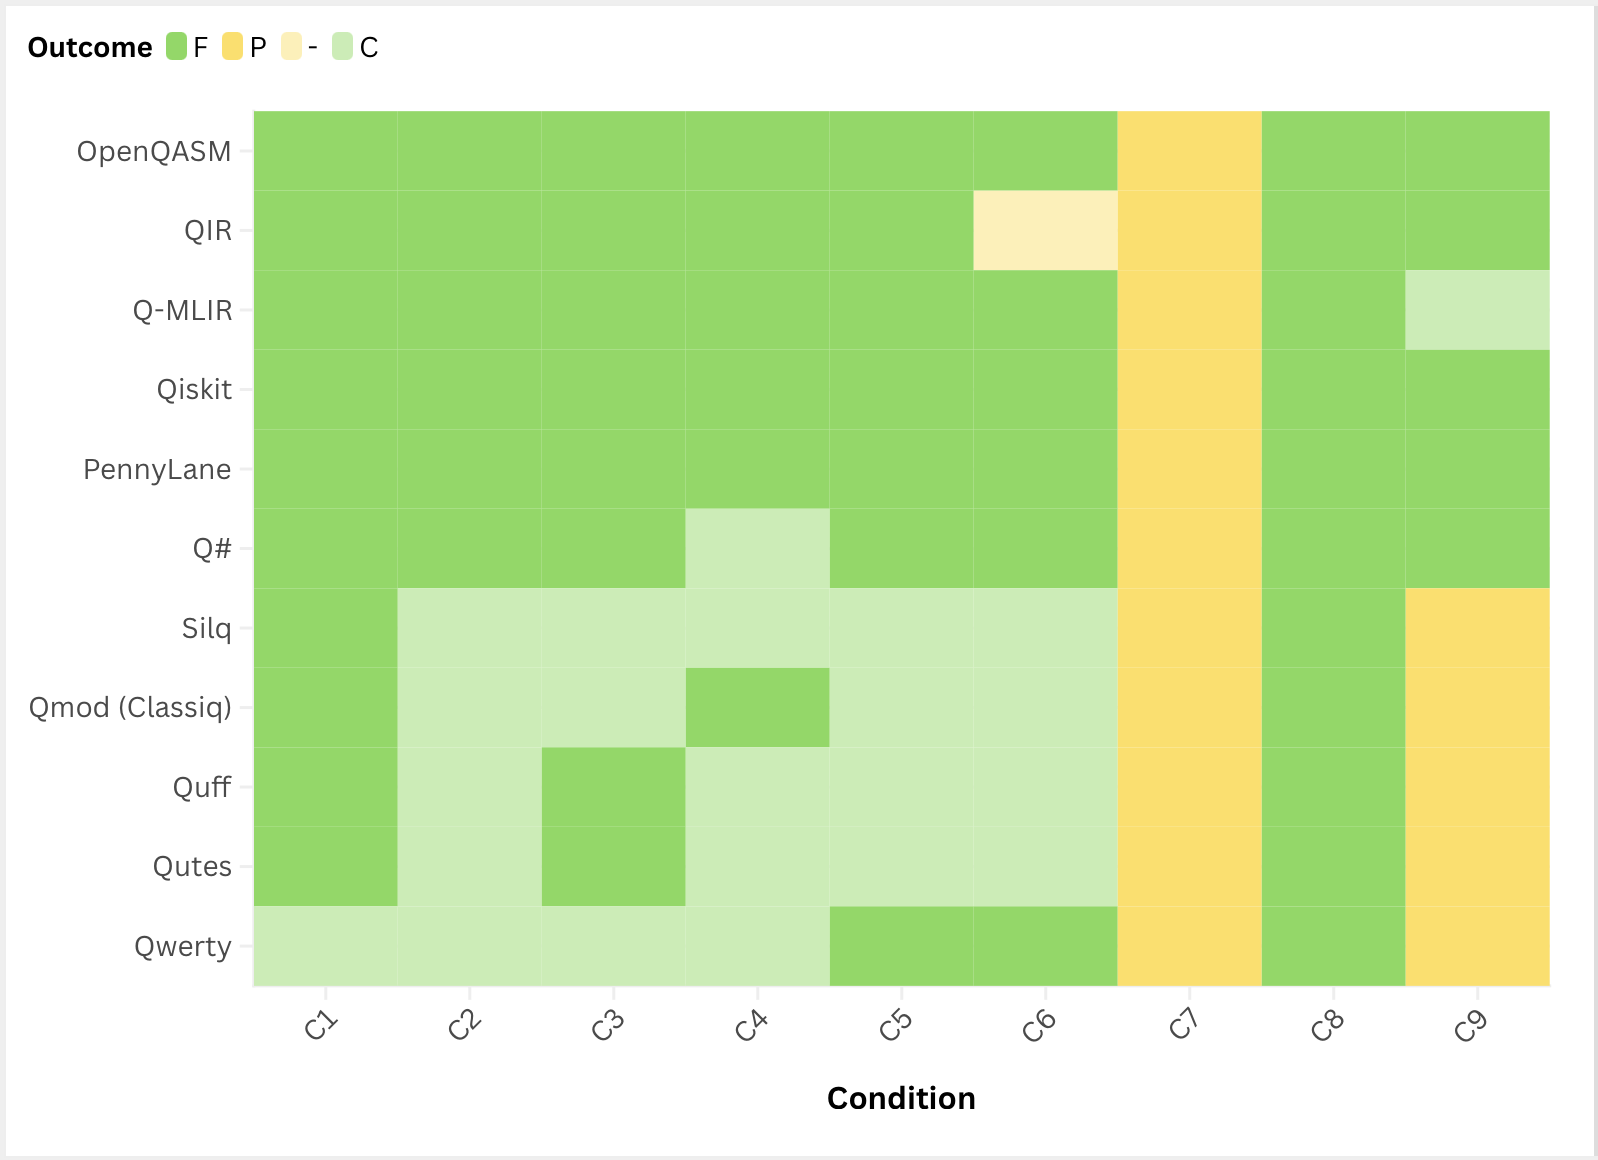
\includegraphics[width=0.95\linewidth]{../../figures/fig-system_assessments-condition_heatmap}
    \caption{Systems $\times$ conditions outcome heatmap (F/C/P/-).}
    \label{fig:system_assessments:condition_heatmap}
\end{figure}
\fi
\section{Discussion}\label{sec:discussion}

\subsection{RQ1: Current abstraction levels and the quantum-implicit gap}\label{subsec:discussion:rq1}
No reviewed system meets the quantum-implicit requirements across the representative task suite, as recorded in Table~\ref{tab:system_assessments:system_summary}.
The recurring constraints concern primary artefacts, qubit identity and observation boundaries.
Their persistence gives the quantum-bias framing in Section~\ref{subsec:introduction:quantum_bias} a task-based evidential basis.

Assembly and IR systems provide instruction fidelity, interchange and compiler-facing representations, while Framework systems provide library abstraction, transpilation and execution infrastructure.
These systems address requirements within their intended roles rather than failing because they retain the representations they were designed to support.
The remaining vocabulary requirement is consistent with accounts of abstraction progress dominated by structure and tooling over circuit substrates~\cite{corralesgarro2025productivityexpressiveness,furntratt2024higherabstractionlevels}.
High-level systems simplify additional obligations but only partially meet the programmer-facing requirements identified in the literature~\cite{DiMatteo2024AbstractionHierarchy,nunez_corrales2025betterabstractmachines}.

Tier assignments do not capture all differences in structured reversal, observation handling and composition.
Q\#, Quff, Qutes and Qwerty provide program-like organisation or alternative expression mechanisms, yet their recorded profiles remain Framework because other obligations persist.

\subsection{RQ2: A new quantum programming language is justified}\label{subsec:discussion:rq2}
OpenQASM, QIR and Q-MLIR retain explicit instruction or compiler representations and resource identities.
Qiskit and PennyLane add library reuse and execution tooling without replacing circuit-oriented authoring.
Q\#'s typed operations and structured reversal and Silq's program-level values and compiler-managed safety simplify construction without eliminating quantum-specific constructs and observation requirements~\cite{MicrosoftQSharpOverview,bichsel2020silq}.

Qmod provides synthesis, Quff runtime inversion and Qutes task-specific implicit operations, improving composition and result extraction without removing every obligation across the suite~\cite{vax2025qmodexpressivehighlevelquantum,wright2024quff,faro2025qutes}.
Qutes' membership operation passes all nine conditions, but that success does not extend across its remaining constructions.
Qwerty's basis-oriented programming changes the authoring representation, yet retains explicit staging, observation and phase reasoning elsewhere in the suite~\cite{adams2024qwerty}.
Its artefact and resource-identity passes in Deutsch--Jozsa and Grover likewise do not extend across the complete task suite.

Required quantum knowledge persists across these authoring models, particularly in phase estimation.
This pattern is consistent with practitioner evidence identifying quantum vocabulary and insufficient higher-level abstraction as adoption barriers~\cite{ferreira2024qplusage}.

Quantum constraints on copying, observation and temporary-value disposal must be respected by the implementation~\cite{yuan2025foundationalabstractions}.
They do not by themselves determine which responsibilities must remain in the programmer's working model.

Tower provides familiar data structures and an associated control machine model while retaining explicit reversibility obligations~\cite{yuan2025foundationalabstractions}.
Its exclusion prevents treating it as a demonstrated quantum-implicit solution, but its design supports considering alternatives to circuit-centred authoring.

Across the assessed tasks, the gap is structural rather than simply a shortage of reusable functions, compiler assistance or higher-level syntax.
A new language that makes quantum realisation an implementation responsibility is therefore justified.
The comparison does not establish that every possible adaptation of an existing system would fail.

\subsection{Methodological reflections}\label{subsec:discussion:methodological_reflections}
OpenQASM's C7 passes despite the expected Assembly profile because the examples do not require timing, topology or pulse-level calibration.
Task under-coverage, examples that avoid hardware-control features or changes in default assembly workflows could explain this outcome.
The recorded pattern does not distinguish those explanations.

QIR's C6 lacks task-aligned observation evidence.
A missing outcome can reflect an unexercised capability, an obligation absent from the artefact or incomplete source coverage.
It must not be interpreted as either satisfied abstraction or demonstrated lack of capability.

\subsection{Design implications}\label{subsec:discussion:implications}
The comparison supports four requirements for a quantum-implicit design, consistent with the abstract-machine concerns identified in the literature~\cite{nunez_corrales2025betterabstractmachines}.

\paragraph{Quantum data model first}
The authoring model should express programs over values, with circuits derived through compilation rather than manipulated as the primary artefact.
Persistent C2 constraints despite improved C9 outcomes distinguish this requirement from modularity alone.
Program-first syntax is insufficient where ordinary use reintroduces qubit identity or explicit observation.

\paragraph{Computation model separation}
The computation model should operate over language abstractions without requiring programmers to name, index or manage implementation qubits.
Safety mechanisms and library conveniences simplify particular obligations, but the recorded identity constraints remain.
Quantum resource guarantees must not make execution-level bookkeeping a prerequisite of representative programming.

\paragraph{Measurement as system policy}
The language and runtime should manage result extraction rather than requiring programmers to select and wire observation into ordinary programs.
A compact measurement builtin reduces bookkeeping but still exposes the observation boundary.
Programs should consume usable results without requiring explicit measurement operations, sampling strategies or observable interfaces.

\paragraph{Vocabulary-free by default, expert access preserved}
The common programming path should permit programs to be written, tested and reasoned about without amplitude, phase or entanglement vocabulary.
Task-dependent C8 failures distinguish this requirement from improved function structure.
Explicit opt-ins should preserve expert access for optimisation, verification and low-level control.
This priority addresses the quantum vocabulary and abstraction barriers identified in practitioner evidence~\cite{ferreira2024qplusage}.
\section{Conclusion}\label{sec:conclusion}
Quantum-implicit entry criteria can be derived from the existing literature.
The eleven assessed systems populate the Assembly, IR, Framework and High-level tiers, but none meets the quantum-implicit requirements across the representative task suite (RQ1).
The persistent gap across the surveyed approaches is structural rather than merely a matter of missing features, justifying a new language targeting this tier (RQ2).

\paragraph{Limitations}
The theoretically grounded instrument has not undergone controlled validation of its condition definitions or the stability of F/C/P judgements across evaluators~\cite{Coblenz2021PLIERS,Myers2016PLUsabilitySIG}.
The findings reflect the field as of 2026-04-08 and do not account for subsequent system developments.
Practitioner evidence discussed in Section~\ref{sec:background} is observational, and a complementary user study would strengthen the design implications independently of instrument validation.
The pre-specified system selection underrepresents photonic computing languages and topological qubit frameworks, limiting generalisation across quantum computing paradigms.
The small, canonically grounded task suite may produce comparative patterns driven by what the examples and available primary-source evidence exercise rather than by systems' full capabilities.

\paragraph{Future work}
Documentation-only learnability studies using T1--T4 would examine required programmer knowledge, while independent inter-rater studies would measure agreement on F/C/P outcomes.
Expanded system sets and domain-specific tasks would test the instrument's coverage and support reconsideration of tier boundaries.
The design implications in Section~\ref{subsec:discussion:implications} motivate a quantum-implicit prototype with optional expert control.
It should be evaluated against the gating constraints in Section~\ref{subsec:evaluation_instrument:conditions} across representative tasks, using the same evidence discipline as this review.


    \printbibliography

\end{document}